\subsection{Complete decision traces and finite-pool risk}
\label{sec:7-budget-trace}

All 2,304 sampled curves are monotone and bisection selects the
enumerated minimum; the twelve FULL calls also pass both checks.
Summing full-pool per-query counts over recorded sample IDs reproduces
all 18,432 grid counts, supporting \cref{eq:6-finite-pool} on these
subsets. This aggregate check does not establish per-query invariance
for arbitrary subsets or positions. The structural grouped-path
guarantee and distance-only exceptions remain those of
\cref{sec:6-3}.

At $S=128$, maxima reach 0.0050 for arXiv/512 and 0.0046 for BGE/512;
at $S=32$ the largest is 0.0294. A low mean loss therefore coexists
with occasional materially worse chosen budgets. FULL's maximum across
the twelve cells remains 0.0006.

For arXiv/128, predicted crossings at $S=32,64,128$ are
0.965/0.875/0.620, versus 0.984/0.875/0.625 observed
(\cref{fig:7-finite-pool}). The largest discrepancy among 36 comparisons
is 0.144 on BGE/512 at $S=128$ (0.519 predicted, 0.375 observed).
Prediction conditions on stable query counts and uses held-out fixed-arm
quality to map accepted budgets to GT loss; the agreement decision itself
uses no labels.

\begin{figure}[tbp]
\centering
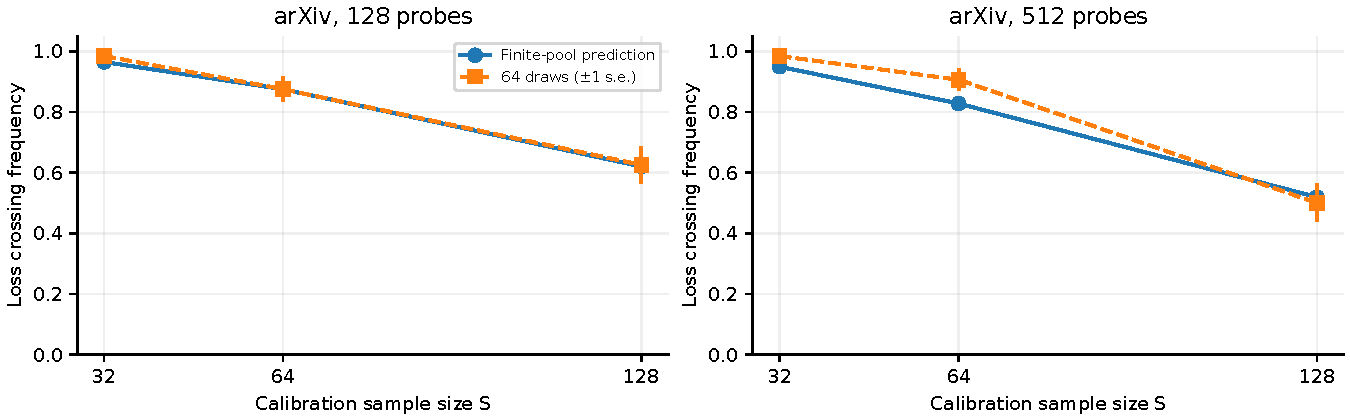
\includegraphics[width=\linewidth]{supplement/finite-pool.pdf}
\caption[Finite-pool risk prediction and observation]{Finite-pool prediction and observed arXiv loss crossings. Bars
show one estimated standard error over 64 independently drawn subsets
conditional on the fixed pool, not uncertainty over future workloads.}
\label{fig:7-finite-pool}
\end{figure}

Ten alternating repetitions resolve the apparent small-budget speed
inversion into a low-budget timing plateau. This observation does not
impose monotone runtime across all budgets and resource transitions.

\subsection{Direct calibration-plus-reuse measurement}
\label{sec:7-stream-cost}

Four cells compare fixed 64/100 with sampled and FULL calibration
over five rotated-policy rounds and 500 held-out batches. The timer
includes gathering, calibration, budget installation and first-batch graph
setup; construction, warm-up and scan calibration are excluded.
The same query pool is replayed (\cref{tab:7-stream-cost}).

\par\medskip\noindent\begin{minipage}{\linewidth}
\centering\captionsetup{hypcap=false}
\captionof{table}[Direct costs for 500 reuse batches]{Direct total milliseconds for 500 reuse batches, averaged over
five rounds, including budget calibration for sampled and FULL policies.
Each batch has 500 queries. Quality is discussed with the timing results.}
\label{tab:7-stream-cost}
\footnotesize\setlength{\tabcolsep}{4pt}
\begin{tabular}{@{}lrrrr@{}}
\toprule
Dataset/probes & Fixed 100 & Fixed 64 & Rule $S=128$ & FULL \\
\midrule
arXiv/128 & 1224 & 1102 & 1291 & 1680 \\
OpenAI-1536/128 & 1491 & 1264 & 852 & 860 \\
OpenAI-3072/128 & 2757 & 2160 & 1769 & 1783 \\
BGE/512 & 5185 & 5018 & 4921 & 5062 \\
\bottomrule
\end{tabular}

\end{minipage}\par\medskip

On OpenAI-3072/128, the sampled policy selects 4 in every round and
reduces total time from 2,757 to 1,769\,ms against fixed 100, about
36\%, at the same measured recall 0.9252. FULL selects the same budget
and takes 1,783\,ms including its larger calibration cost. On
OpenAI-1536/128, FULL takes 860 versus 1,491\,ms at the same recall
0.9280; the sampled policy averages 852\,ms and 0.9276 recall.

Measured mean cumulative savings first appear at 4/6 batches on
OpenAI-1536 and 4/9 on OpenAI-3072 against fixed 100/64
(\cref{fig:7-stream-cost}); fractional steady-rate fits are separate
model estimates. BGE/512 trades lower time for lower mean recall:
4,921 versus 5,185\,ms and 0.9658 versus 0.9670 for sampled/fixed 100.
FULL reaches 0.9664 at 5,062\,ms. ArXiv's FULL policy selects 200 for
quality and is slower than fixed 100/64, which miss the target.
Calibration's benefit therefore depends jointly on quality and total
reuse cost.

\begin{figure}[tbp]
\centering
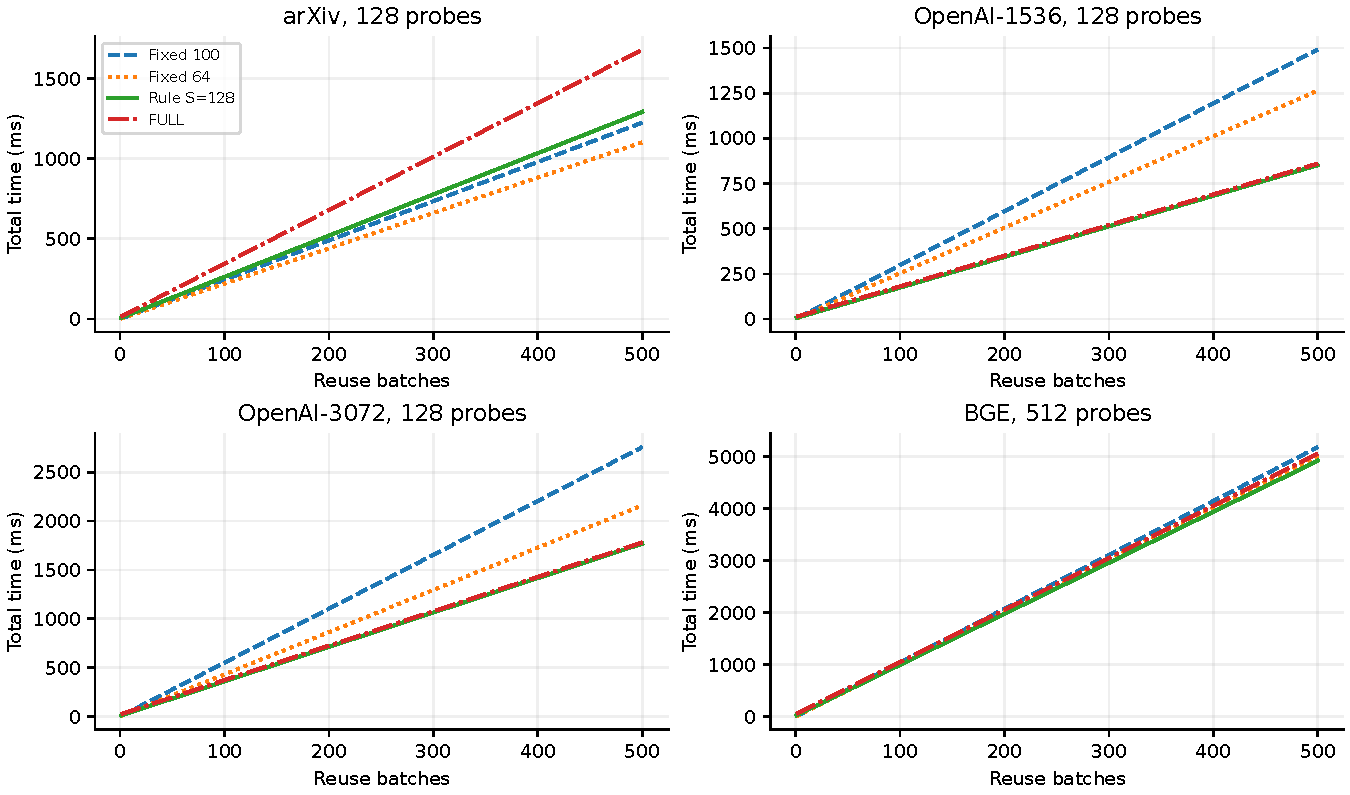
\includegraphics[width=\linewidth]{supplement/stream-cost.pdf}
\caption[Direct cumulative calibrated-reuse time]{Direct mean cumulative time, including budget calibration and
first-batch setup. Each curve replays one fixed held-out query pool.
Policies can have different recall; timings alone are not a quality-matched
ranking. Dataset/probe settings match \cref{tab:7-stream-cost}.}
\label{fig:7-stream-cost}
\end{figure}
